\documentclass[tikz,border=10pt]{standalone}
\usepackage{tikz}
\usetikzlibrary{arrows, shapes.geometric, decorations.markings}

\begin{document}

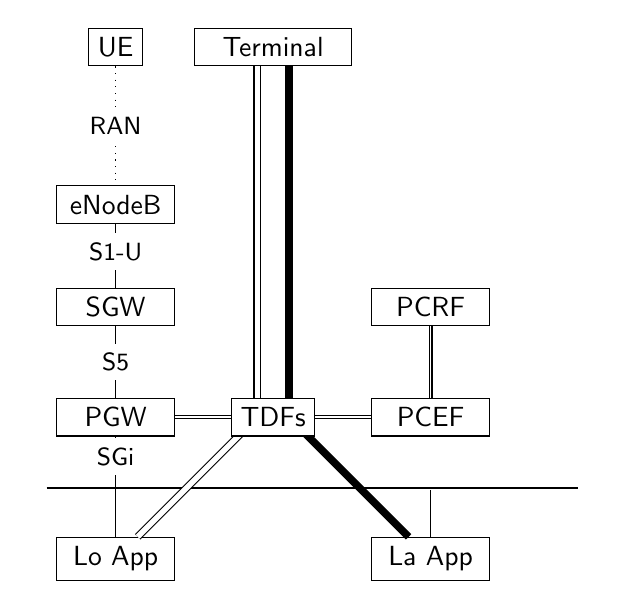
\begin{tikzpicture}[auto, node distance=2cm,>=latex']
    \tikzstyle{iface}=[font=\small\sffamily]
    \tikzstyle{elem}=[font=\sffamily]
  \node (ue) at (0,0) [elem,draw,rectangle] {UE};
  \node (l) at (2,0) {}; % invisible node
  \node (l1) at (1.8,0) {}; % invisible node
  \node (l2) at (2.2,0) {}; % invisible node
  \node (eb) at (0,-2) [elem,draw,rectangle, minimum width=1.5cm]{eNodeB};
  \node (sgw) at (0,-3.3) [elem,draw,rectangle, minimum width=1.5cm] {SGW};
  \node (pgw) at (0,-4.7) [elem,draw,rectangle, minimum width=1.5cm] {PGW};
  \node (k) at (2,-4.7) {}; % invisible node
  \node (k1) at (1.8,-4.7) {}; % invisible node
  \node (k2) at (2.2,-4.7) {}; % invisible node
  \node (pcef) at (4,-4.7) [elem,draw,rectangle, minimum width=1.5cm] {PCEF};
  \node (pcrf) at (4,-3.3) [elem,draw,rectangle, minimum width=1.5cm] {PCRF};

  %% SGi LAN
  \node (a) at (-1,-5.6) {}; % invisible node
  \node (b) at (6,-5.6) {}; % invisible node
  \node (c) at (0,-5.6) {}; % invisible node
  \draw[black] (a) -- (b);
  %% \draw[black] (-0.5,-5.6) -- (6,-5.6);
  %% \draw[black] (a) to (b);

%  \node (loa) at (2,-6.5) [draw,rectangle]{Lo App};
  \node (app) at (0,-6.5) [elem,draw,rectangle, minimum width=1.5cm]{Lo App};
  \node (d)   at (0,-5.5) {}; % invisible node
  \node (laa) at (4,-6.5) [elem,draw,rectangle, minimum width=1.5cm]{La App};
  \node (e)   at (4,-5.5) {}; % invisible node


  \draw[black] (eb) to (sgw);
  \draw[black] (sgw) to (pgw);
  \draw[black] (pgw) to (app);
  %% \draw[black] (pgw) to (c);
  %% \draw[black] (d) to (app);
  \draw[black] (e) to (laa);

  \draw[double] (pgw) to (pcef);
  \draw[double] (pcrf) to (pcef);
  \draw[dotted] (ue) to (eb);% {RAN} (ran);

%  \draw [black,thin,double distance=2pt,double=gray]  (l) to (k);
  \draw [black,thin,double distance=2pt,double=white] (l1) to (k1);
  \draw [black,thin,double distance=2pt,double=black] (l2) to (k2);
  \draw [black,thin,double distance=2pt,double=white] (k1) to (app);
%  \draw [black,thin,double distance=2pt,double=gray]  (k) to (loa);
  \draw [black,thin,double distance=2pt,double=black] (k2) to (laa);

  \node (tdfs) at (2,-4.7) [elem,draw,rectangle,fill=white] {TDFs};
  \node (apps) at (2,0)    [elem,draw,rectangle,fill=white, minimum width=2cm] {Terminal};
  \node (sgi) at (0,-1)    [iface,draw=white,fill=white]{RAN};
  \node (sgi) at (0,-5.2)  [iface,draw=white,fill=white]{SGi};
  \node (s1u) at (0,-2.6)  [iface,draw=white,fill=white]{S1-U};
  \node (s5) at (0,-4)     [iface,draw=white,fill=white]{S5};

  % Note: If you have no branches, the 2nd pass is not needed
\end{tikzpicture}

\end{document}
